% Нумерация страниц
\setcounter{page}{2}

\subsection*{Цель}

Знакомство со средством дизассемблирования – sourcer и с
получением дизассемблерного кода ядра операционной системы Windows на примере обработчика прерывания INT 8h в virtual mode – специальном режиме защищенного режима, который эмулирует реальный режим работы вычислительной системы на базе процессоров Intel.

\section*{Листинг кода}

\subsection*{Листинг INT 8h}

\begin{lstlisting}[style={asm}]
; Вызов подпрограммы sub_1.
020A:0746  E8 0070				call	sub_1			; (07B9)

; Сохранение содержимого регистров ES, DS, AX, DX.
020A:0749  06					push	es
020A:074A  1E					push	ds
020A:074B  50					push	ax
020A:074C  52					push	dx

; Загрузка в регистр DS 40h.
020A:074D  B8 0040				mov	ax,40h
020A:0750  8E D8				mov	ds,ax

; Загрузка в регистр ES 00h.
020A:0752  33 C0				xor	ax,ax			; Zero register
020A:0754  8E C0				mov	es,ax

; Инкремент счетчика таймера.
020A:0756  FF 06 006C				inc	word ptr ds:[6Ch]	; (0040:006C=4FBAh)
; Проверка счетчика таймера == 0.
020A:075A  75 04				jnz	loc_1			; Jump if not zero

; Инкремент старшей части счетчика таймера.
020A:075C  FF 06 006E				inc	word ptr ds:[6Eh]	; (0040:006E=11h)

020A:0760			loc_1:						;  xref 020A:075A
; Сравнение cтаршей части счетчика таймера с 24.
020A:0760  83 3E 006E 18			cmp	word ptr ds:[6Eh],18h	; (0040:006E=11h)
020A:0765  75 15				jne	loc_2			; Jump if not equal

; Сравнение младшей части счетчика таймера с 176.
020A:0767  81 3E 006C 00B0			cmp	word ptr ds:[6Ch],0B0h	; (0040:006C=4FBAh)
020A:076D  75 0D				jne	loc_2			; Jump if not equal

; Обнуление счетчика таймера.
020A:076F  A3 006E				mov	word ptr ds:[6Eh],ax	; (0040:006E=11h)
020A:0772  A3 006C				mov	word ptr ds:[6Ch],ax	; (0040:006C=4FBAh)

; Загрузка 1 по адресу 0000:0470h,
; если прошло более 24 часов с момента запуска таймера.
020A:0775  C6 06 0070 01			mov	byte ptr ds:[70h],1	; (0040:0070=0)
020A:077A  0C 08				or	al,8

020A:077C			loc_2:						;  xref 020A:0765, 076D
; Сохранение регистра AX.
020A:077C  50					push	ax
; Декремент времени, оставшегося до отключения моторчика дисковода.
020A:077D  FE 0E 0040				dec	byte ptr ds:[40h]	; (0040:0040=44h)
; Проверка счетчика таймера == 0.
020A:0781  75 0B				jnz	loc_3			; Jump if not zero
; Установка флага, необходимого для отключения моторчика дисковода.
020A:0783  80 26 003F F0			and	byte ptr ds:[3Fh],0F0h	; (0040:003F=0)
; В порт - команду отключения моторчика дисковода.
020A:0788  B0 0C				mov	al,0Ch
020A:078A  BA 03F2				mov	dx,3F2h
020A:078D  EE					out	dx,al			; port 3F2h, dsk0 contrl output

020A:078E			loc_3:						;  xref 020A:0781
; Восстановление регистра AX.
020A:078E  58					pop	ax
; Проверка флага PF.
020A:078F  F7 06 0314 0004			test	word ptr ds:[314h],4	; (0040:0314=3200h)
020A:0795  75 0C				jnz	loc_4			; Jump if not zero
; Сохранение младшего байта регистра FLAGS в AH.
020A:0797  9F					lahf				; Load ah from flags
020A:0798  86 E0				xchg	ah,al
; Сохранение регистра AX.
020A:079A  50					push	ax
; Косвенный вызов 1Ch.
020A:079B  26: FF 1E 0070			call	dword ptr es:[70h]	; (0000:0070=6ADh)
020A:07A0  EB 03				jmp	short loc_5		; (07A5)
020A:07A2  90					nop

020A:07A3			loc_4:						;  xref 020A:0795
; Вызов прерывания 1Ch.
020A:07A3  CD 1C				int	1Ch			; Timer break (call each 18.2ms)

020A:07A5			loc_5:						;  xref 020A:07A0
; Вызов подпрограммы sub_1.
020A:07A5  E8 0011				call	sub_1			; (07B9)
; Сброс контроллера прерываний.
020A:07A8  B0 20				mov	al,20h			; ' '
020A:07AA  E6 20				out	20h,al			; port 20h, 8259-1 int command
										;  al = 20h, end of interrupt

; Восстановление регистров DX, AX, DS, ES.
020A:07AC  5A					pop	dx
020A:07AD  58					pop	ax
020A:07AE  1F					pop	ds
020A:07AF  07					pop	es

; Переход в адрес 020A:064C.
020A:07B0  E9 FE99				jmp	$-164h
;...
020A:06AC  CF					iret				; Interrupt return
\end{lstlisting}

\clearpage

\subsection*{Листинг sub\_1}

\begin{lstlisting}[style={asm}]
			   sub_1       proc    near
; Сохранение содержимого регистров DS, AX.
020A:07B9  1E					push	ds
020A:07BA  50					push	ax

; Загрузка в регистр DS 40h.
020A:07BB  B8 0040				mov	ax,40h
020A:07BE  8E D8				mov	ds,ax

; Сохранение младшего байта регистра FLAGS в AH.
020A:07C0  9F					lahf				; Load ah from flags

; Проверка флага DF == 0. Проверка старшего бита IOPL == 0.
020A:07C1  F7 06 0314 2400			test	word ptr ds:[314h],2400h	; (0040:0314=3200h)
020A:07C7  75 0C				jnz	loc_2			; Jump if not zero

; IF = 0 в 0040:0314h.
020A:07C9  F0> 81 26 0314 FDFF	           lock	and	word ptr ds:[314h],0FDFFh	; (0040:0314=3200h)

020A:07D0			loc_1:						;  xref 020A:07D6
; Загрузка содержимого AH в младший байт регистра FLAGS. 
020A:07D0  9E					sahf				; Store ah into flags

; Восстановление регистров AX, DS.
020A:07D1  58					pop	ax
020A:07D2  1F					pop	ds
020A:07D3  EB 03				jmp	short loc_ret_3		; (07D8)

020A:07D5			loc_2:						;  xref 020A:07C7
; IF = 0. Запрет прерываний от внешних устройств.
020A:07D5  FA					cli				; Disable interrupts
020A:07D6  EB F8				jmp	short loc_1		; (07D0)

020A:07D8			loc_ret_3:					;  xref 020A:07D3
; Возврат из подпрограммы.
020A:07D8  C3					retn
sub_1       endp
\end{lstlisting}

\clearpage

\section*{Схемы алгоритмов}

%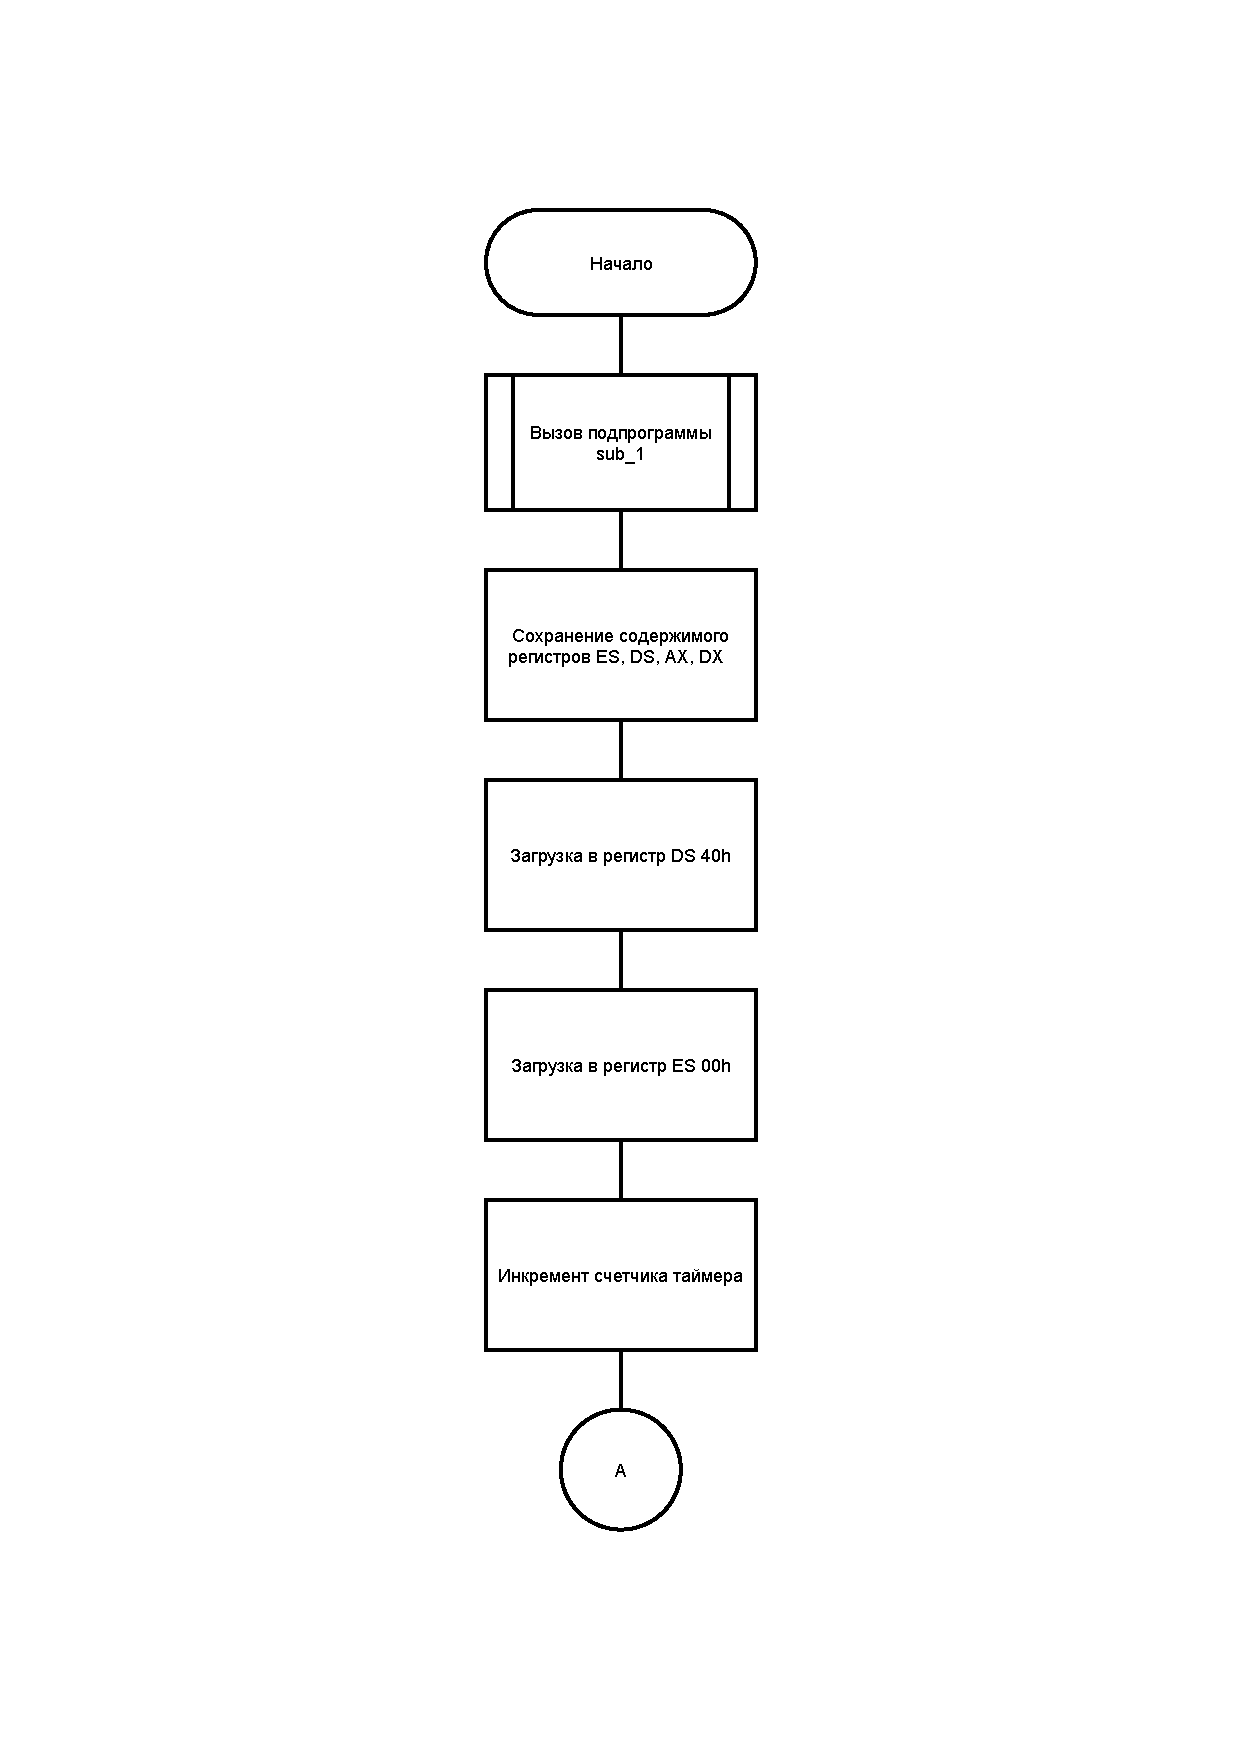
\includepdf[pages=1,scale=.8,pagecommand={\section*{Схемы алгоритмов}\label{pdf:8h}},linktodoc=true]{8h.pdf}
%\includepdf[pages=2-,scale=.8,pagecommand={},linktodoc=true]{8h.pdf}
\img{220mm}{8h_1.png}{Схема обработчика прерываний INT 8h}

\img{220mm}{8h_2.png}{Схема обработчика прерываний INT 8h}

\img{220mm}{8h_3.png}{Схема обработчика прерываний INT 8h}

\img{220mm}{8h_4.png}{Схема обработчика прерываний INT 8h}

\img{220mm}{sub_1.png}{Схема подпрограммы sub\_1}

\clearpage

